\documentclass[11pt,a4paper]{article}
\usepackage[T1]{fontenc}
\usepackage[utf8]{inputenc}
\usepackage{lmodern,microtype}
\usepackage{amsmath,amssymb,amsthm,mathtools}
\usepackage{booktabs,array,longtable,graphicx,float,xcolor}
\usepackage[margin=2.05cm]{geometry}
\usepackage{enumitem,fancyhdr,hyperref}
\hypersetup{unicode=true,colorlinks=true,linkcolor=blue!45!black,urlcolor=blue!55!black,
 pdftitle={FIN ST432--ST446: Sector Exclusion, Certified Orbit Census, and Infrared Degree},
 pdfauthor={Krzysztof Żuchowski},
 pdfsubject={Finite analytical and computational continuation of FIN},
 pdfkeywords={FIN, strict kernel, entropy, gain transition, Krawczyk, Brouwer degree, Morse theory, invariant theory}}
\pagestyle{fancy}\fancyhf{}\lhead{FIN ST432--ST446}\rhead{Release 10.86}\cfoot{\thepage}
\setlength{\headheight}{14pt}
\newcommand{\Proven}{\textcolor{green!38!black}{\textbf{[PROVEN]}}}
\newcommand{\Evidence}{\textcolor{orange!80!black}{\textbf{[STRONG NUMERICAL EVIDENCE]}}}
\newcommand{\Partial}{\textcolor{orange!80!black}{\textbf{[PARTIAL]}}}
\newcommand{\Blocked}{\textcolor{red!65!black}{\textbf{[BLOCKED]}}}
\newtheorem{theorem}{Theorem}
\newtheorem{proposition}{Proposition}
\newtheorem{corollary}{Corollary}

\title{\textbf{FIN ST432--ST446}\\[3pt]
Sector Exclusion, a Certified Stationary-Orbit Census,\\
and Local Infrared Degree\\[6pt]
\large Release 10.86}
\author{Krzysztof \.{Z}uchowski\\
\small Independent Researcher --- Fractal Information Theory Project\\
\small ORCID: 0009-0002-0909-3613}
\date{14 August 2026}

\begin{document}
\maketitle

\begin{abstract}
Programs ST432--ST446 continue the local analytical and computational FIN
program after Release 10.85.  The main global-variational advance is a rigorous
two-sector exclusion at every supplied gain $g\le2.88$.  No negative
competitor to the uniform state exists when
$\max_i p_i\le0.14824732498$ or when $\max_i p_i\ge0.8$; any missed
competitor must lie in the explicit intermediate band.  This does not close
the global transition.  The already certified reflection-even branch crosses
the uniform energy transversely in the narrow ST342 interval, with
$dV/dg\in[-0.671281367,-0.671275547]$, but exclusion of a third competitor
remains open.

The singular infrared continuation is strengthened substantially.  One common
parametric Krawczyk box now proves a unique compactified root for every
$b=1/y_3\in[0,0.017]$, an $8.5$-fold extension.  On $b\in[0,0.015]$ a uniform
contraction certificate fixes the Jacobian orientation and proves local
Brouwer degree $-1$.  Separately, symmetry-averaged interval boxes determine
the exact stabilizers of nine previously isolated stationary representatives.
Their $D_{12}$ orbits contain $85$ distinct certified stationary points.  The
partial Morse polynomial is $13+42t+30t^2$ and is already Euler-balanced,
$13-42+30=1$, although completeness and heteroclinic connections are not
proved.

The batch also excludes all degree-eight invariant syzygies of support at most
two over two primes, closes the characteristic-zero degree-five primitive
quotient at dimension $52$, improves synthetic E- and A-optimal design metrics
with one exchange, sharpens a numerical transfer-gap sequence, and enlarges a
conservative local input-to-state stability ball.  No result derives the gain,
selects one orbit member, supplies dimensional units, completes a
legacy-to-strict physical-role transfer, or adds external empirical evidence.
\end{abstract}

\tableofcontents
\newpage

\section{Scope, source packet, and nonclaims}

The audited repository baseline is Git commit
\texttt{bb540a767e210a5a3bf816e4868e7bcefbac3872}, supplemented by the
uncommitted local ST417--ST431 packet and the executable artifacts listed in
the reproducibility section.  The strict finite operator is
\begin{equation}\label{eq:A}
 A=sI-W,\qquad W_{xx}=0,\qquad
 W_{xy}=\frac{\cos(0.18575d(x,y)+0.16250)}{1+d(x,y)^{9/5}}\quad(x\ne y),
\end{equation}
on $\mathbb Z_{12}$, with off-diagonal row sum
$s=1.660307278766099\ldots$.  The supplied variational family is
\begin{equation}\label{eq:V}
 V_g(p)=D(p\Vert u)-\frac g2q^TAq,\qquad
 q=p-u,\quad u_i=\frac1{12},\quad
 D(p\Vert u)=\sum_i p_i\log(12p_i).
\end{equation}
All quantities below are dimensionless.

The legacy ontological kernel remains an intermediate bridge kernel.  It is
not silently identified with \eqref{eq:A}; no legacy electroweak,
electromagnetic, gravity-hierarchy, Planck-scale, or other physical role is
transferred.  The project ontology is retained only as context: the nadsoliton
itself is primordial fractal information in a solitonic state---there is no
separate informational layer below it---with the preferred internal order
nadsoliton $\to$ light $\to$ matter $\to$ emergent observer.

A $D_{12}$ orbit is not a selector.  QW-2191 remains open.  A theorem
conditional on $g$ does not source $g$.  A dimensionless optimization branch
is not a physical infrared phenomenon, and local computation is not external
validation.

\section{Executive result ledger}
\small
\begin{longtable}{>{\raggedright\arraybackslash}p{.075\textwidth}>{\raggedright\arraybackslash}p{.19\textwidth}>{\raggedright\arraybackslash}p{.63\textwidth}}
\toprule Program&Status&Result\\\midrule\endhead
ST432&\Proven{} limited&Over each of two primes, all 2028 degree-eight candidates are nonzero and pairwise nonproportional; support-one/two syzygies are excluded.  The forced 136-dimensional relation problem remains unsolved.\\
ST433&\Proven{} partial&For $g\le2.88$, negative competitors are excluded in the uniform and concentrated outer sectors; the band $0.1482473<\max p_i<0.8$ remains open.\\
ST434&\Proven{} local&The certified reflection-even equal-value crossing is transverse and locally unique in gain; global third-competitor exclusion is absent.\\
ST435&\Proven{} nonexhaustive&Exact stabilizers and orbit sizes certify 85 distinct stationary points generated by the nine isolated representatives.\\
ST436&\Proven{} census / \Partial{} topology&The partial Morse polynomial is $13+42t+30t^2$ and has Euler sum one.  Completeness and Conley connections remain open.\\
ST437&\Proven&A common Krawczyk box proves unique singular attachment for every $b\in[0,0.017]$.\\
ST438&\Proven{} local&On $b\in[0,0.015]$, $\|I-CJ\|_\infty\le0.938101<1$ and the branch component has Brouwer degree $-1$.\\
ST439&\Proven{} bounded&The characteristic-zero degree-five primitive quotient has dimension $52$; degree six is bounded between $39$ and $55$, not closed.\\
ST440&\Evidence&One weakest-direction row exchange improves the synthetic E metric by $4.29\%$ and the A metric by $4.16\%$.\\
ST441&\Proven{} cone bound / \Evidence{} spectrum&Five Ulam grids stabilize near a modulus ratio $0.595740$; no infinite-dimensional two-sided gap bracket is proved.\\
ST442&\Proven{} conditional&A paid local ISS ball has radius $1.93\times10^{-6}$ and forcing threshold $4.2163\times10^{-5}$.\\
ST443&\Blocked&Mixed rank-seven edge signs still defeat the positive-weight envelope; no certified sign-aware SDP closure is obtained.\\
ST444&\Blocked&No internal strict source of $g$ is exported.\\
ST445&\Blocked&No nonpremise selector is exported; QW-2191 remains open.\\
ST446&\Blocked&No independent referee, laboratory record, custody chain, or held-out empirical datum is added.\\
\bottomrule
\end{longtable}
\normalsize

\section{ST433--ST434: what is now known about the gain transition}

For $p\ne u$ with $q^TAq>0$, equality $V_g(p)=V_g(u)=0$ occurs at
\begin{equation}\label{eq:ratio}
 g(p)=\frac{2D(p\Vert u)}{q^TAq}.
\end{equation}
Consequently the first possible global change satisfies the exact variational
identity
\begin{equation}\label{eq:gc}
 g_{\mathrm c}=\inf_{p\ne u}\frac{2D(p\Vert u)}{q^TAq}.
\end{equation}
This reformulates the unresolved problem as a global ratio minimization; it
does not assume the known local branch is the minimizer of \eqref{eq:gc}.

\subsection{Uniform sector}

Let $\lambda_{\max}(A)=2.342182041146301\ldots$.  If
$\max_i p_i\le m$, then on the tangent space
\[
 \nabla^2V_g(p)=\operatorname{diag}(1/p_i)-gA
 \succeq(1/m-g\lambda_{\max})I.
\]
Thus the convex sector containing $u$ has no negative competitor whenever
$m\le1/(g\lambda_{\max})$.  At $g=2.88$ this gives
\begin{equation}\label{eq:mconv}
 \max_i p_i\le0.14824732498259885.
\end{equation}

\subsection{Concentrated sector}

Write the largest coordinate as $1-t$, normalize the other eleven to a vector
$y$, and put $\rho=\sum_jy_j^2$.  Entropy extremization at fixed $\rho$, a
feasible SOCP-dual water-fill lower bound for the center-to-remainder energy,
and the smallest strict edge weight give a two-variable lower envelope.
A $1000\times1000$ outward-paid cover of
\[
 0\le t\le0.2,\qquad 1/11\le\rho\le1
\]
has minimum lower bound
\begin{equation}\label{eq:margin}
 V_{2.88}(p)\ge0.005770490891026778.
\end{equation}
The computation pays $10^{-10}$ per cell for floating roundoff, far below the
displayed margin.  The gain term is monotone, so the same exclusion holds for
every $g\le2.88$.

\begin{theorem}[Two-sector exclusion]
At every supplied $g\le2.88$, no negative competitor exists in either
\[
 \max_i p_i\le0.14824732498259885
 \quad\text{or}\quad
 \max_i p_i\ge0.8.
\]
Any unobserved negative competitor must lie in the intermediate band.
\end{theorem}

This is not a global transition theorem: the intermediate band remains
eleven-dimensional and is not covered.

\subsection{Transversality of the known branch}

ST342 certifies a unique reflection-even stationary tube for
\[
 g\in[2.902496471747767,2.9024964917477667].
\]
Along a stationary branch, the envelope theorem gives
\[
 \frac{d}{dg}V_g(p(g))=-\frac12q(g)^TAq(g).
\]
Outward evaluation on the complete tube gives
\[
 q^TAq\in[1.3425510931,1.3425627340],
 \quad
 \frac{dV}{dg}\in[-0.6712813670,-0.6712755465].
\]
Hence the branch crossing is transverse and unique inside the tube.  A third
global competitor is not excluded.

\section{ST435--ST436: exact orbit sizes and the Morse shadow}

The full dihedral group has order $24$.  For each of the nine ST421 roots,
the center was averaged over its numerical stabilizer and a new invariant
radius-$2.1\times10^{-9}$ Krawczyk box was certified.  Uniqueness inside an
invariant box proves that the exact root has the declared stabilizer.  Every
nonstabilizing transform is separated by at least $0.1373$ in one coordinate,
many orders of magnitude more than the box diameter.

\begin{center}
\begin{tabular}{c|rrrrrrrrr}
\toprule representative&O0&O1&O2&O3&O4&O5&O6&O7&O8\\\midrule
stabilizer order&2&24&2&4&2&4&2&2&2\\
orbit size&12&1&12&6&12&6&12&12&12\\
Morse index&0&0&1&1&1&2&1&2&2\\\bottomrule
\end{tabular}
\end{center}

\begin{proposition}[Certified nonexhaustive census]
The nine local representatives generate $85$ distinct stationary points of
the supplied $g=4$ functional.  Their index counts are
\[
 m_0=13,\qquad m_1=42,\qquad m_2=30.
\]
\end{proposition}

Their partial Morse polynomial and alternating sum are
\begin{equation}\label{eq:morse}
 M_{\mathrm{partial}}(t)=13+42t+30t^2,
 \qquad M_{\mathrm{partial}}(-1)=1.
\end{equation}
The value one equals the Euler characteristic of the simplex.  This is a
striking internal consistency check, not a completeness proof: further
critical points can occur in index-canceling families, and boundary-stratified
Morse bookkeeping has not been completed.

\begin{figure}[H]\centering
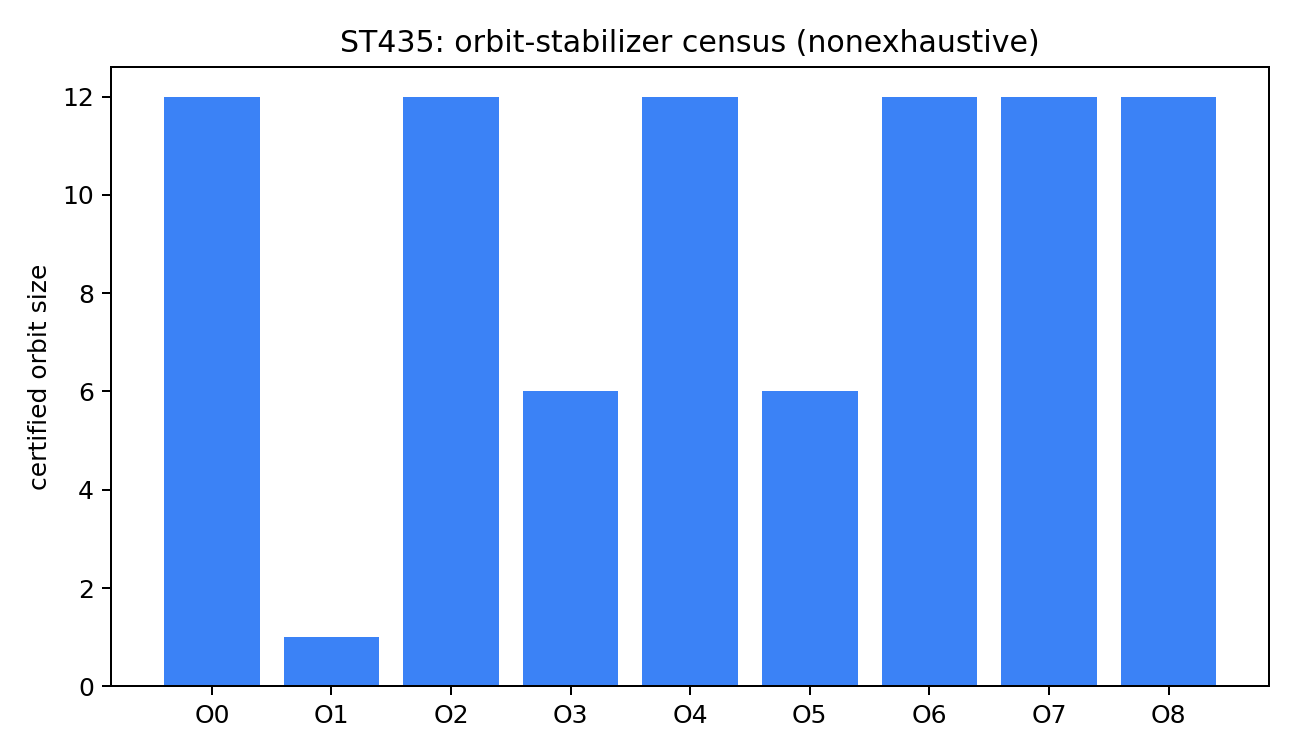
\includegraphics[width=.76\textwidth]{FIN_ST432_ST446_Figures/st435_orbit_sizes.png}
\caption{Certified orbit sizes for the nine isolated representatives.  The figure does not assert that the atlas is exhaustive.}
\end{figure}

\section{ST437--ST438: an enlarged singular attachment and local degree}

The compactification remains
\[
 b=1/y_3,\qquad c=ay_3,\qquad a=bc,
\]
with exponentially flat tails extended by zero at $b=0$.  A common five-box
for $(y_1,y_2,c,\nu,T)$ is centered at the $b=0.0085$ root.  Its radii are
chosen from the endpoint variation and then verified, rather than trusted, by
the Krawczyk inclusion.  On the complete interval $b\in[0,0.017]$ the smallest
component margin is
\[
 1.7121949701\times10^{-7}>0.
\]
In the box-scaled infinity norm, the associated derivative contraction is
$0.159774<1$, which separately pays uniqueness throughout the tube.

\begin{theorem}[Extended compactified attachment]
For every $b\in[0,0.017]$, the regularized five-equation system has exactly one
root in the displayed common box.  At $b=0$ it is the certified limiting face;
for $b>0$ it is the original finite-$y_3$ root.  This extends the prior
$b\le0.002$ result by a factor $8.5$.
\end{theorem}

The same fixed-box construction fails at $b=0.018$.  That failure is not a
fold, band loss, or no-go; it only marks the limit of this box template.

For $b\le0.015$, interval left multiplication by the midpoint inverse gives
\[
 \sup\|I-CJ\|_\infty\le0.9381006921<1.
\]
All Jacobians in the box are therefore nonsingular and homotopic through
nonsingular matrices to the midpoint Jacobian, whose determinant is
$-0.5667433846\ldots$.

\begin{corollary}[Local degree]
The unique compactified branch component has local Brouwer degree $-1$ for
every $b\in[0,0.015]$.
\end{corollary}

This is a local component theorem.  It does not exclude additional components
outside the box and it does not provide a dimensional infrared scale.

\section{ST432 and ST439: invariant-algebra progress and the exact boundary}

The degree-eight candidate family contains $2028$ formal products in an
invariant space of dimension $1892$, so at least $136$ relations are forced.
At each of the primes $1000003$ and $1000033$, ST432 evaluates all candidates
at $128$ exact mean-zero points, projectively normalizes every nonzero
signature, and hashes the complete signatures.  There are no zero signatures
and no projective duplicates.

\begin{proposition}
No rational degree-eight syzygy in the declared candidate family has support
one or two.
\end{proposition}

Indeed, a primitive rational two-term relation reduces nontrivially modulo
either prime and would force proportional signatures.  The proposition gives
a sparsity obstruction; it does not find any of the support-three-or-higher
relations.

For the joint odd/even presentation, both primes give decomposable ranks
\[
 \operatorname{rank}R_5^{\rm dec}=72,
 \qquad \operatorname{rank}R_6^{\rm dec}=310.
\]
A nonzero modular minor is a nonzero integer minor, hence supplies a lower
rank bound over $\mathbb Q$.  Candidate counts supply upper bounds.  Because
there are exactly $72$ degree-five candidates, the characteristic-zero rank
is exactly $72$ and the primitive quotient dimension is
\[
 124-72=52.
\]
At degree six there are $326$ candidates, so only
\[
 39\le\dim Q_6^{\rm primitive}\le55
\]
is proved over characteristic zero.  Agreement of two primes does not prove
the missing upper rank bound.

\section{ST440--ST443: design, transfer, nonlinear basin, and rank seven}

\subsection{A one-exchange design improvement}

The frozen pool has $1800$ synthetic mean-zero observations and $365$ sextic
coefficients.  Starting from the prior 500-row pivoted-QR design, the weakest
right-singular direction selects one excluded row and removes the selected row
with smallest response in that direction.  One exchange changes
\[
 \sigma_{\min}:1.64404393\times10^{-4}
 \longrightarrow1.71457251\times10^{-4},
\]
an E-improvement factor $1.042899$.  The A criterion
$\operatorname{tr}(X^TX)^{-1}$ improves by factor $1.041606$, and the condition
number falls from $14758.8$ to $14132.5$.  These are deterministic numerical
design facts for a synthetic pool, not a measurement apparatus.

\subsection{Transfer gap}

The certified Birkhoff contraction remains the theorem-level bound.  Bilinear
Ulam grids of side $21,31,41,51,61$ give a second/first modulus ratio ending at
\[
 0.5957429137,\qquad0.5957401632,
\]
with last-step difference $2.75\times10^{-6}$.  The convergence is strong
evidence for the synthetic fixture.  A collectively compact approximation
error is still missing, so these values are not an infinite-dimensional
spectral-gap bracket.

\begin{figure}[H]\centering
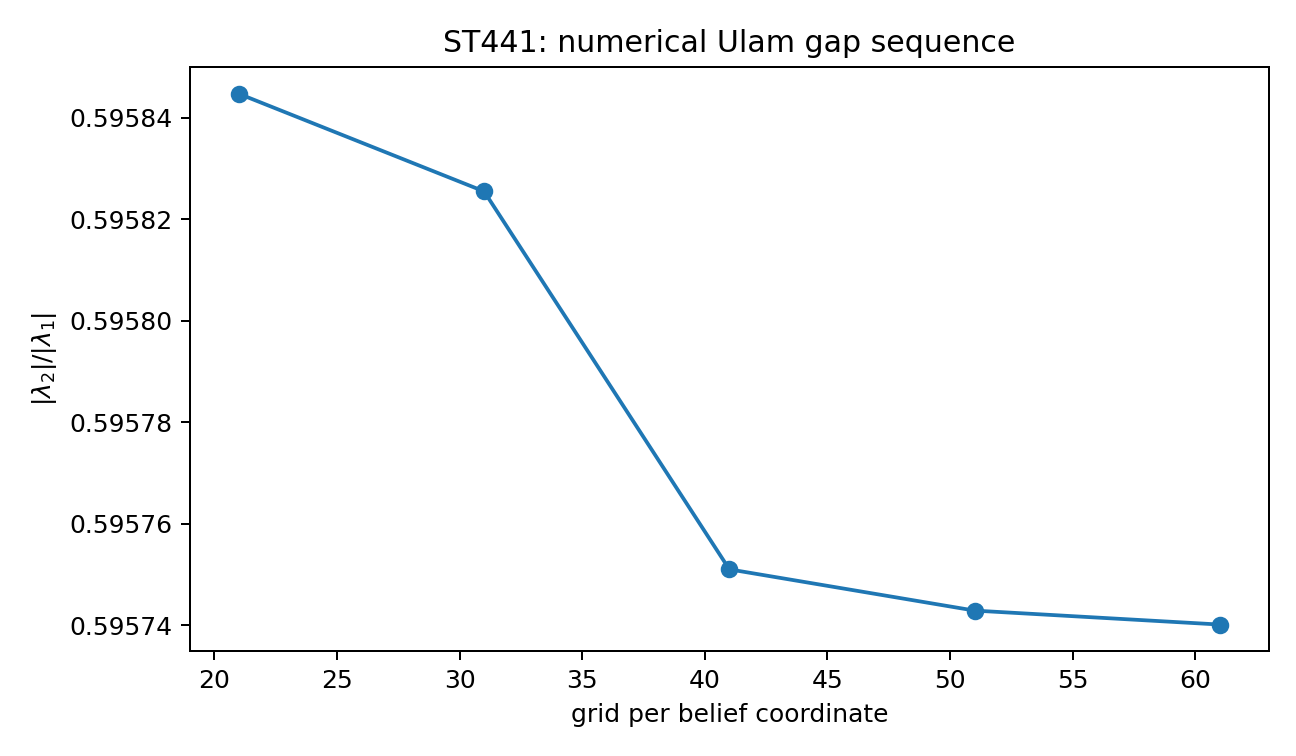
\includegraphics[width=.76\textwidth]{FIN_ST432_ST446_Figures/st441_ulam_ratio.png}
\caption{Finite-grid transfer ratios.  The plotted convergence is numerical; the cone bound remains the rigorous statement.}
\end{figure}

\subsection{Optimized conservative ISS ball}

For the localized minimum, use the paid Hessian-variation estimate
\[
 \mu(R)=\mu_0-\frac{R}{(p_{\min}-R)^2}.
\]
Choosing $R=1.93\times10^{-6}$ yields $\mu\ge43.69210566$ and admissible
tangent forcing
\[
 \epsilon<\frac{\mu R}{2}=4.21628819\times10^{-5}.
\]
Relative to ST427, the certified radius grows by $1.93$ and the forcing
threshold by $1.309$.  The result remains local, conditional, and
dimensionless.

\subsection{Rank-seven stop}

The rank-seven mediator has the same maximal eigenvalue as $A$ but contains
$24$ positive and $42$ negative off-diagonal pairs.  The strict positive-edge
water-fill argument is therefore unavailable.  No local certified SDP solver
is installed, and no independent rational SDP dual was constructed.  The
global rank-seven variational claim remains blocked; spectral coincidence is
not positivity-geometry equivalence.

\section{What survives falsification}

The batch supports four conclusions and no stronger ones.

\begin{enumerate}[leftmargin=1.6em]
\item The global transition problem is now localized in probability space,
but the intermediate band prevents identification of its critical gain.
\item The singular IR branch is a genuine unique compactified component over a
much larger interval and has certified local orientation.  Its global topology
and physical interpretation remain open.
\item The known stationary landscape is richer than a list of nine numerical
points: it contains 85 interval-certified points with an unexpectedly balanced
partial Morse census.  The balance is not an exhaustion theorem.
\item The invariant algebra has a real characteristic-zero result at degree
five and a real sparsity obstruction at degree eight.  The full relation basis
is still missing.
\end{enumerate}

The deepest surviving interpretation is therefore still operator-theoretic
and variational: a supplied strict finite spectral object supports a controlled
entropy--quadratic phase family, a compactifiable singular optimization
component, and a structured invariant algebra.  These are mathematically
coherent shadows of a common finite object.  They do not yet constitute a
theorem from primordial information to dimensional, experimentally testable
physics.

\section{Recommended programs ST447--ST461}

\begin{longtable}{>{\raggedright\arraybackslash}p{.08\textwidth}>{\raggedright\arraybackslash}p{.65\textwidth}>{\raggedright\arraybackslash}p{.16\textwidth}}
\toprule Program&Acceptance test&Priority\\\midrule\endhead
ST447&Use checkpointed sparse Wiedemann/Lanczos algebra to recover support-$\ge3$ degree-eight modular relations.  Lift across two primes and verify each integer polynomial identity directly.&1\\
ST448&Cover the unresolved band $0.1482473<\max p_i<0.8$ at successive gain slabs by interval branch-and-bound with entropy and quadratic relaxations.  Accept only a full simplex certificate.&1\\
ST449&If ST448 isolates one global crossing, certify equality, transversality, and exclusion of every third competitor.  This is the gate for a unique global critical gain.&1\\
ST450&Construct an interval cover of a full $D_{12}$ fundamental domain for the stationary equations.  Determine whether the 85-point census is exhaustive.&1\\
ST451&Build isolating blocks or a Conley connection matrix for the index-one saddles.  Do not promote finite-time trajectories.&2\\
ST452&Continue the IR branch beyond $b=0.017$ with overlapping adaptive boxes and boundary matching; isolate a genuine fold only if interval singularity conditions pass.&2\\
ST453&Complete the IR complement cover, including root ordering, inactive slack, derivative signs, and exponential-tail exclusion.&2\\
ST454&Find exact characteristic-zero degree-six relations, then combine them with ST447 into a minimal joint odd/even presentation through degree eight.&2\\
ST455&Run multi-exchange E/A/D optimization on a frozen training pool and report all metrics on a separately frozen synthetic hold-out pool.&3\\
ST456&Prove a collectively compact Ulam error estimate and convert the transfer sequence into two-sided leading/second spectral-value brackets.&2\\
ST457&Replace the local ISS ball by a certified larger sublevel basin or prove a sharp obstruction caused by the simplex boundary.&2\\
ST458&Implement a sign-aware rank-seven SDP relaxation with a rational dual replay.  Accept only a paid bound that closes the localization/curvature gap.&2\\
ST459&Re-run the strict gain-source admission gate only if ST447--ST458 export a genuinely new typed source object; otherwise preserve the block.&Gate\\
ST460&Re-run selector/QW-2191 only if a nonpremise symmetry-breaking provider is exported; orbit counting alone is inadmissible.&Gate\\
ST461&Keep the evidence gate closed until an independent record, custody split, frozen hold-out, and preregistered analysis exist.&Gate\\
\bottomrule
\end{longtable}

\section{Reproducibility packet}

The executable source is \texttt{fin\_st432\_st446\_research.py}.  It writes
15 per-program JSON packets, \texttt{FIN\_ST432\_ST446\_Results.json}, a CSV
ledger, and two figures.  The test suite
\texttt{test\_fin\_st432\_st446.py} contains 15 tests, including live replay
of the degree-eight signature audit and the enlarged IR Krawczyk certificate;
all pass.  The SHA-256 manifest covers the source, packets, ledger, figures,
tests, TeX source, and final PDF.

\medskip
\noindent\textbf{Epistemic final line.}  This release adds proof-grade local
mathematics and explicitly bounded numerical evidence.  It adds no physical
unit, selector, laboratory fact, Standard Model/gravitation derivation, or
Theory-of-Everything closure.

\end{document}
